\begin{figure}
\begin{center}
    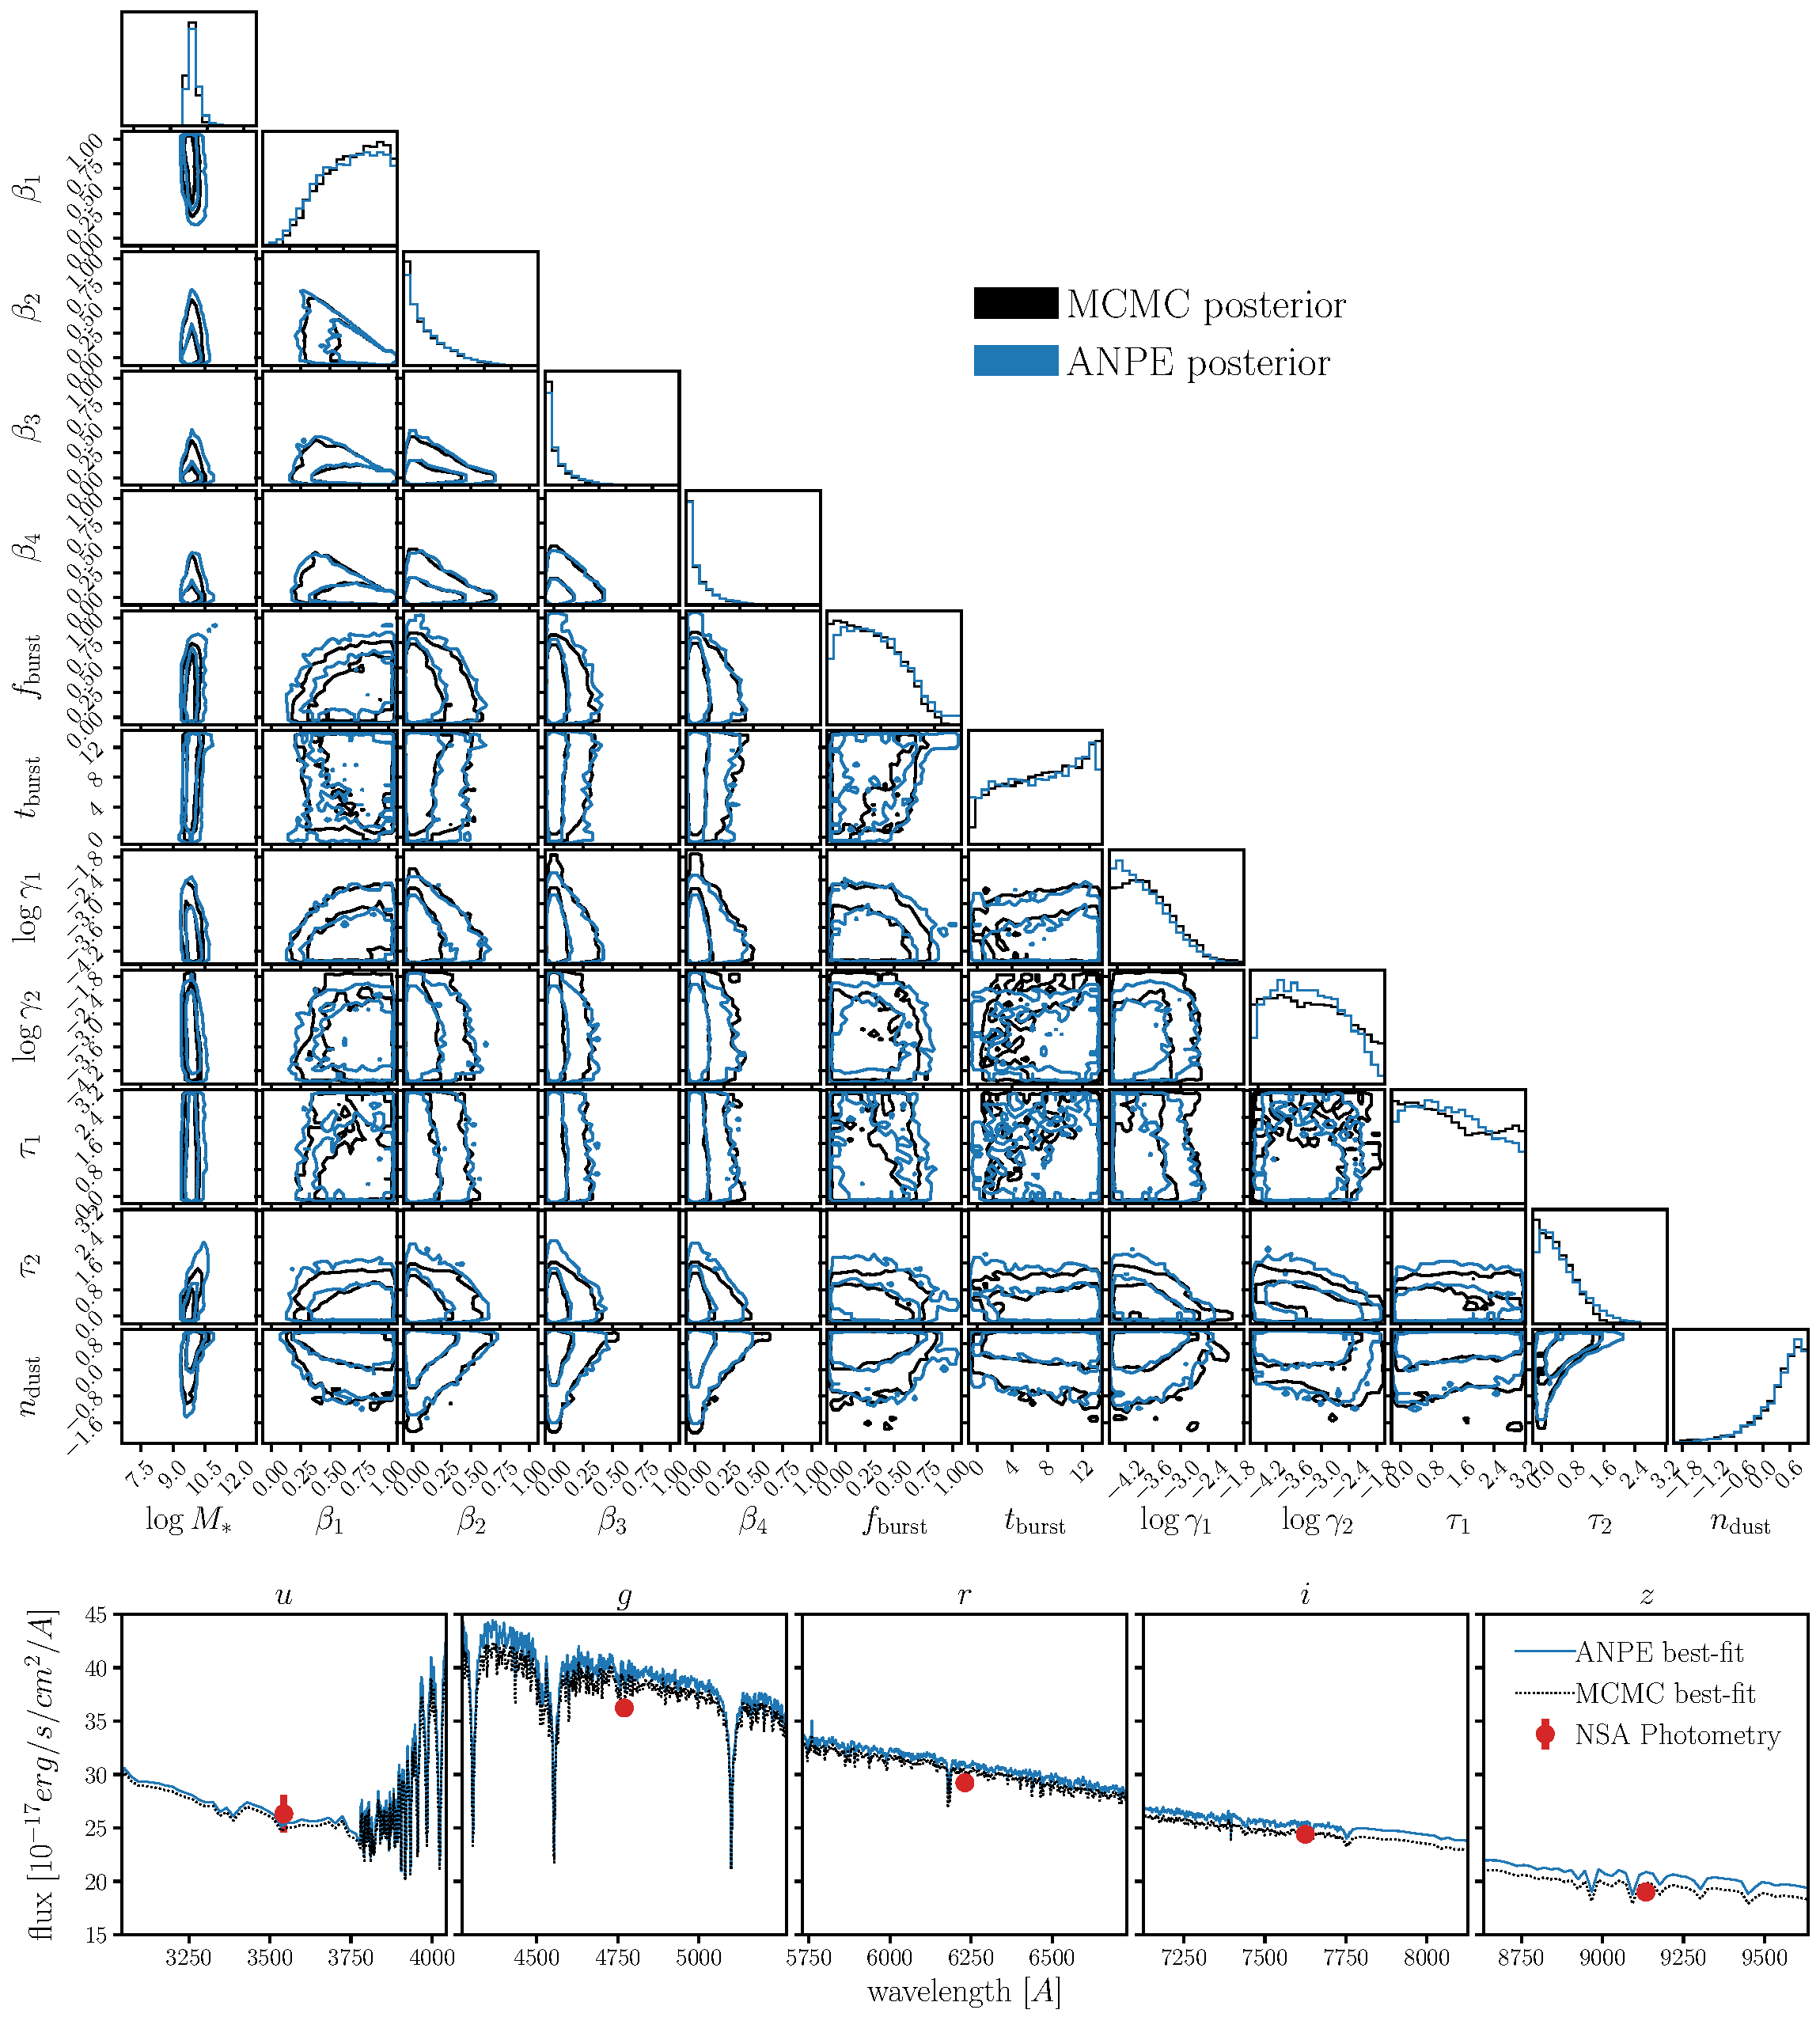
\includegraphics[width=0.9\textwidth]{figs/corner.pdf}
    \caption{\label{fig:corner}
    A comparison of the posteriors of the 12 SED model parameters derived from
    standard MCMC sampling (black) and our \sedflow~(blue) for an arbitrarily
    selected NSA galaxy.
    The posteriors are in excellent agreement for all of the SED parameters. 
    In the bottom panel, we present the SEDs of the the best-fit parameter
    values from the \sedflow~(blue) and MCMC posteriors (black dotted), which
    are all in excellent agreement with the observed NSA photometric flux
    (red). 
    We mark the optical broadband response curves (dashed) for reference. 
    Estimating the posterior using MCMC sampling requires 10 CPU hours. 
    Even using neural emulators to accelerate likelihood evaluations, MCMC
    sampling requires 10 CPU minutes. 
    \emph{With \sedflow, inferring the full posterior takes 1 second per
    galaxy.}
    }
\end{center}
\end{figure}

\section{Results} \label{sec:results}
Now that we have trained \sedflow, we can estimate the posterior,
$p(\theta\given \bfi{x}_i)$, for any $\bfi{x}_i = \{f_X, \sigma_X, z \}$. 
In pratice, we do this by drawing samples from the \sedflow~NDE model:
$q(\theta\given \bfi{x}_i, {\bf h})$. 
Since we use a normalizing flow, this is trivial:
we generate samples from the target distribution of the normalizing flow,  a
multivariate Gaussian distribution in our case, then we transform the samples
using the bijective transformation in Eq.~\ref{eq:normflow} that we trained.
The transformed samples follow $q(\theta\given \bfi{x}_i, {\bf h})$ and 
estimates the posterior, $p(\theta\given \bfi{x}_i)$. 

Next, we validate the accuracy of the \sedflow~posterior estimates, before we
apply it to the NSA sample.
As a first test, we compare the posterior from \sedflow~to the posterior derived
from MCMC sampling for a single arbitrarily chosen NSA galaxy in
Figure~\ref{fig:corner}. 
In the top, we present the the posterior distribution of the 12 SED model
parameters (Section~\ref{sec:provabgs}) for the \sedflow~posterior (blue) and
MCMC posterior (black). 
\emph{The \sedflow~posterior is in excellent agreement with the MCMC posterior
for all of the SED parameters}. 
 
In the bottom of Figure~\ref{fig:corner}, we compare the SEDs of the best-fit
parameter values from the \sedflow~(blue) and MCMC posteriors (black dotted). 
We also include the NSA photometric flux of the selected galaxy (red) and mark
the optical broadband response curves (dashed) for reference. 
The best-fit SED from the \sedflow~posterior is also in excellent agreement
with both the MCMC best-fit SED and the NSA photometry.  

% separate paragraph highlighting the computational advantage? 
The key advantage of ANPE is that it enables accurate Bayesian inference
orders of magnitude faster than conventional methods. 
We derive the MCMC posterior using the {\sc Zeus} ensemble
slice-sampler~\citep{karamanis2020} with 30 walkers and 10,000 iterations.
2,000 of the iterations are discarded for burn-in. 
In total, the MCMC posterior requires >100,000 SED model evaluations. 
Since each evaluation takes ${\sim}340$ ms, it ${\sim}10$ CPU hours for
a single MCMC posterior. 
Recently, SED modeling has adopted neural emulators to accelerate SED model
evaluations~\citep{alsing2020}. 
In \chedit{Hahn~\etal~(2022)}, for instance, the PROVABGS emulator takes
only ${\sim}2.9$ ms to evaluate, >100$\times$ faster than the original model. 
Yet, even with emulators, due to the number of evaluations necessary for
convergence, an MCMC posterior takes ${\sim}10$ CPU minutes. 
Meanwhile, after training, \emph{the \sedflow~posterior takes $1$ second ---
>$10^4\times$ faster than MCMC}. 

\begin{figure}
\begin{center}
    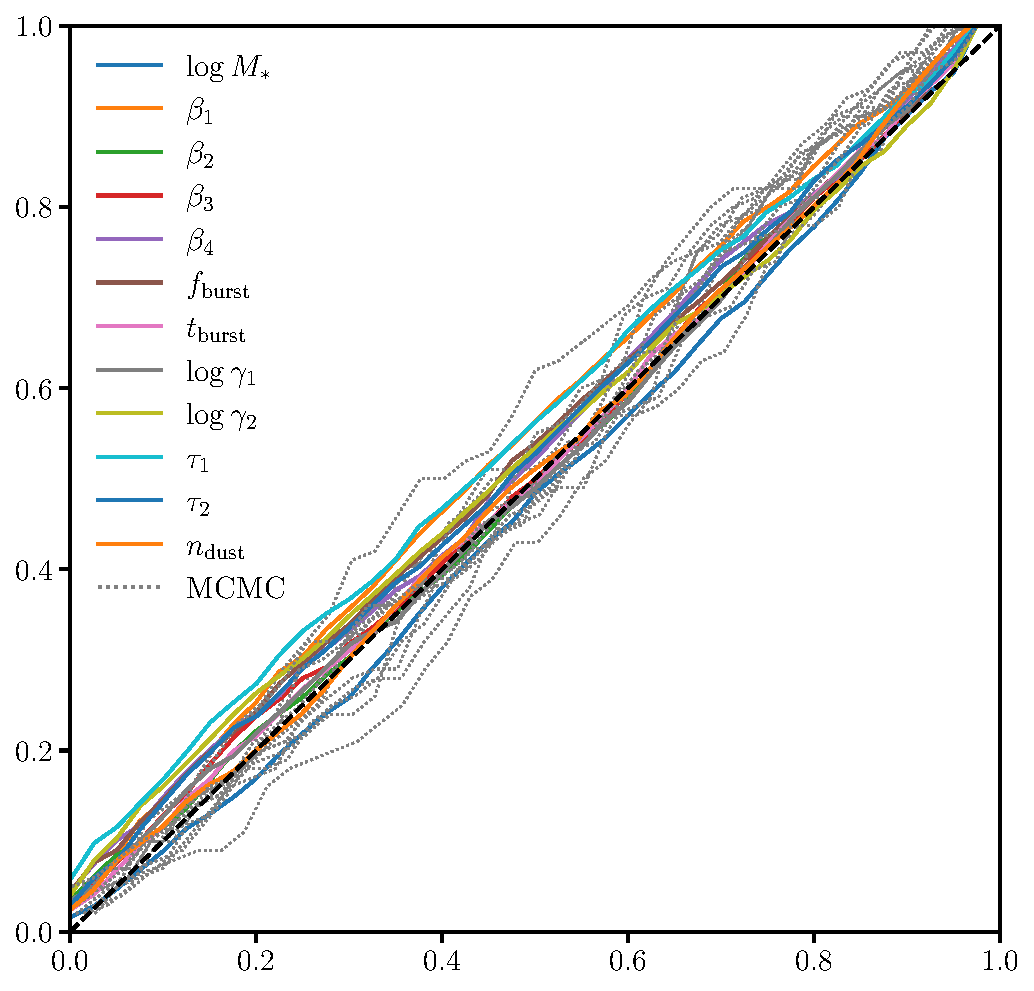
\includegraphics[width=0.5\textwidth]{figs/ppplot.pdf}
    \caption{\label{fig:pp}
    Probability-probability (p-p) plot of the \sedflow~posteriors for 1000
    synthetic test observations, with known true parameter values. 
    We plot the CDFs of the percentile score of the true values within the
    marginalized \sedflow~posteriors for each SED parameter.
    For the true posteriors, the percentile score is uniformly distributed so
    the CDF is diagonal (black dashed).
    The test data is constructed in the same way as the training data
    (Section~\ref{sec:training}). 
    For reference, we include the p-p plot of the posterior estimated from MCMC
    sampling (gray). 
    \emph{The \sedflow~posteriors are in excellent agreement the true
    posteriors.}
    }
\end{center}
\end{figure}
In addition to the NSA galaxy in Figure~\ref{fig:corner}, the posteriors from
\sedflow~and MCMC are overall in excellent for NSA galaxies.
However, we do not know the true SED parameters for these galaxies so to
further validate \sedflow, we use test synthetic photometry, where we know the
truth.
We sample 1000 SED parameters from the prior,
$\{\theta^{\rm test}_i\} \sim p(\theta)$, 
and forward model synthetic NSA observations, 
$\{\bfi{x}^{\rm test}_i\}$, 
for them in the same way as the training data (Section~\ref{sec:training}). 
Afterwards, we generate posteriors for each of $\bfi{x}^{\rm test}_i$ using 
\sedflow: $\{ p(\theta \given \bfi{x}^{\rm test}_i)\}$. 

In Figure~\ref{fig:pp}, we present the probability-probability (p-p) plot of
the \sedflow~posteriors for the test data. 
The p-p plot presents the cumulative distribution function (CDF) of the
percentile score of the true value within the marginalized posterior for each
parameter. 
For true posteriors, the percentiles are uniformly distributed so the CDF is a
diagonal (black dashed).
Overall, the CDFs for \sedflow~lie close to the diagonal for each of the SED
parameters. 
\emph{Hence, the \sedflow~posteriors are in excellent agreement with the true
posteriors}.

In Figure~\ref{fig:pp}, we also include the CDFs of the SED parameters for the
MCMC posteriors derived for a subset of 100 test observations (gray dotted). 
Comparing the CDFs from the MCMC posteriors to those of \sedflow, we find that
the \sedflow~posteriors are actually in better agreement with the true
posteriors. 
This is due to the fact that MCMC posteriors are also only estimates of the
true posterior and are subject to limitations in initialization, sampling, and
convergence.
On the other hand, posteriors from \sedflow~are not impacted by these
limations, so the comparison highlights additional advantages of an ANPE
approach besides the ${>}10^4\times$ speed up.

\begin{figure}
\begin{center}
    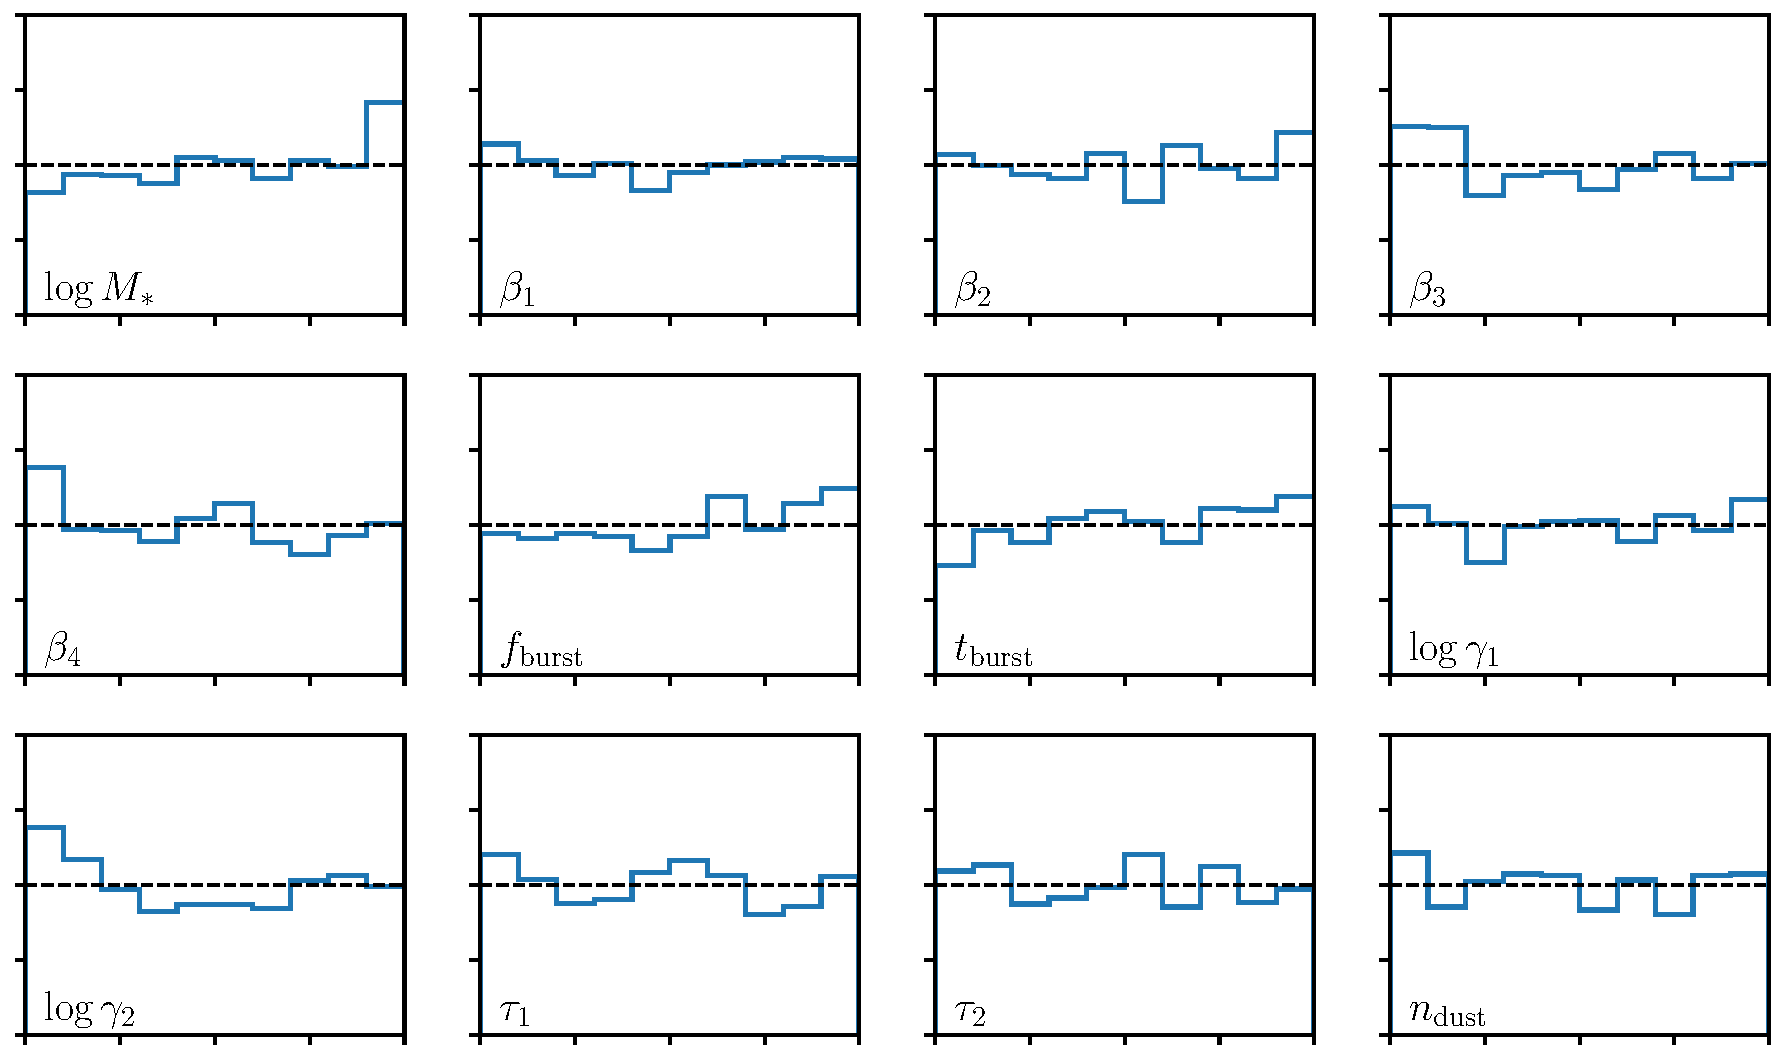
\includegraphics[width=0.9\textwidth]{figs/sbc.pdf}
    \caption{\label{fig:sbc}
    Simulation-based calibration plot of the \sedflow~posteriors for 1000
    synthetic test observations. 
    The histogram in each panel represents the distribution of the rank
    statistic of the true value within the marginalized \sedflow~posterior
    (blue) for each SED parameter.
    For the true posterior, the rank statistics will have a uniform
    distribution (black dashed). 
    For reference, we include the rank distribution of the MCMC posteriors for
    a subset of 100 test data (gray dotted). 
    The rank statistic distribution of \sedflow~is nearly uniform for all of
    the SED parameters. 
    Therefore, \emph{\sedflow~provides unbiased and precise estimates of the
    true posteriors.}
    }
\end{center}
\end{figure}

We examine another validation of the \sedflow~posteriors using simulation-based
calibration~\citep[SBC;][]{talts2020}. 
Rather than using percentile scores, SBC examines the distribution of the rank
statistics of the true parameter values within the marginalized posteriors. 
It addresses the limitation that the CDFs only asymptotically approach the true
values and that the discrete sampling of the posterior can cause artifacts in
the CDFs. 
In Figure~\ref{fig:sbc}, we present SBC of each SED parameter for the
\sedflow~posteriors (blue) using the 1000 test observations.
For comparison, we include the SBC for the MCMC posteriors (gray dotted). 
Similar to the percentile score, the distribution of the rank statistic is
uniform for the true posterior (black dashed). 
The rank statistic distribution for the \sedflow~posteriors are nearly uniform
for all SED parameters. 
Hence, \emph{we confirm that the \sedflow~posteriors are in excellent agreement
with the true posterior}.

An advantage of SBC is that by examining the deviation of rank statistics
distribution from uniformity, we can determine how the posterior estimates
deviate from the true posteriors. 
For instance, if the distribution has a U-shape where the true parameter values
are more often at the lowest and highest ranks, then the posterior estimates
are narrower than the true posteriors.
If the distribution has a $\cap$-shape, then the posterior estimates are
broader than the true posteriors. 
Any asymmetry in the distribution implies that the posterior estimates are
biased.  
For the \sedflow~posteriors, we find none of these features for any of the SED
parameters. 
Hence, \sedflow~provides unbiased and precise estimates of the true posteriors
for all SED parameters. 

With the accuracy \sedflow~validated, we apply it to derive posteriors for all
of our NSA galaxies (Section~\ref{sec:obs}). 
Analyzing all 33,887 NSA galaxies takes \chedit{X} CPU hours. 
For each galaxy, we generate 10,000 samples of the 12-dimensional posterior,
$p(\theta | \xobs)$. 
These posteriors on SED parameters represent posteriors on stellar mass, SFH,
ZH, and dust content of the NSA galaxies. 
To maximize the utility of the posteriors further, we use them to derive
posteriors on the following additional galaxy properties: SFR averaged over
1Gyr, mass-weighted metallicity, and mass-weighted stellar age. 
\chedit{We refer readers to Section X of \cite{hahn2022} for the exact
calculation.}
We publicly release all of the posteriors for our NSA sample at 
\url{some-url-here}. 
Furthermore, \sedflow~model and all of the software used to train it are
publicly available at \url{https://github.com/changhoonhahn/SEDflow/}. 
